\documentclass[tikz,border=4pt]{standalone}
%\usepackage{enumerate}
\usepackage{comment}
\usepackage{graphicx,graphics}
\usepackage{amsfonts}
\usepackage{amssymb}
\usepackage{amsthm}
\usepackage{amsmath}
\usepackage[mathscr]{eucal}
\usepackage[table,dvipsnames]{xcolor}
\usepackage{multirow, array} %para las tablas
%\usepackage{colortbl}
\usepackage{hyperref}
%\usepackage[spanish]{babel} %para el lenguaje español
\usepackage[utf8]{inputenc} %para codificacion lenguaje

\usepackage{xcolor}

%%%%% Paquetes César
\usepackage{subcaption} 
%\captionsetup[subfigure]{labelfont=rm}
\usepackage{float}
\usepackage{booktabs}
\usepackage{orcidlink}

%%%%% Paquetes Dibujos
\usepackage{tikz}
\usetikzlibrary{positioning, arrows.meta}
\usepackage{tkz-euclide}
%\usetkzobj{all}	% With tkz-euclide 3.02, \usetkzobj{all} (or \usetkzobjall) is not necessary according to the manual	

\definecolor{verde}{HTML}{63CAA7}
\definecolor{amarillo}{HTML}{FFC172}
\definecolor{azul}{HTML}{26798E}

\usepackage{pgfplots}
\pgfplotsset{compat=1.18}	%Utilizamos la versión reciente de compatibilidad
\pgfplotsset{ejes1/.append style={axis x line=middle, axis y line=
middle, xlabel={$d_{a,b}$}, ylabel={$\mathscr{P}^r_{a,b}$}}}
\pgfplotsset{ejes2/.append style={axis x line=middle, axis y line=
middle, xlabel={$d_{a,b}$}, ylabel={$\mathscr{A}^r_{a,b}$}}}



\begin{document}

% DIAPO 1.1: 

\begin{comment}
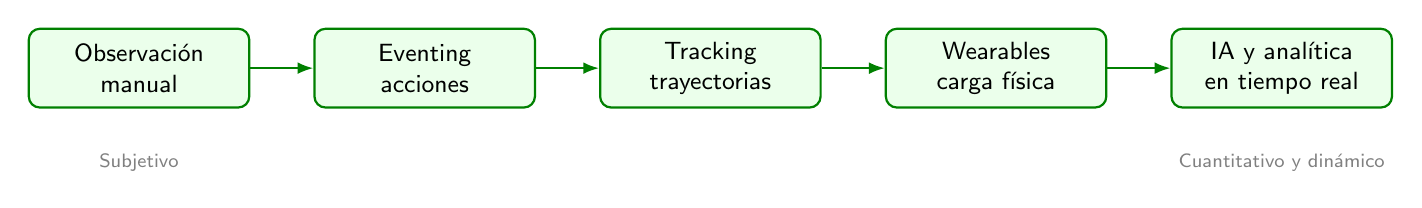
\begin{tikzpicture}[
	node distance=1.2cm and 0.8cm,
	evol/.style={
		rectangle,
		rounded corners=4pt,
		draw=green!50!black,
		thick,
		fill=green!8,
		minimum width=2.8cm,
		minimum height=1.0cm,
		align=center,
		font=\sffamily\small
	},	
	flecha/.style={
		-{Latex[length=2mm]},
		thick,
		green!50!black
	}
	]
	\node[evol] (obs) {Observación\\manual};
	\node[evol, right=of obs] (event)
	{Eventing\\acciones};
	\node[evol, right=of event] (track)
	{Tracking\\trayectorias};
	\node[evol, right=of track] (wear)
	{Wearables\\carga física};
	\node[evol, right=of wear] (ai)
	{IA y analítica\\en tiempo real};
	\draw[flecha] (obs) -- (event);
	\draw[flecha] (event) -- (track);
	\draw[flecha] (track) -- (wear);
	\draw[flecha] (wear) -- (ai);
	\node[
	font=\sffamily\scriptsize,
	text=gray,
	below=0.45cm of obs
	]
	{Subjetivo};
	\node[
	font=\sffamily\scriptsize,
	text=gray,
	below=0.45cm of ai
	]
	{Cuantitativo y dinámico};
\end{tikzpicture}
\end{comment}

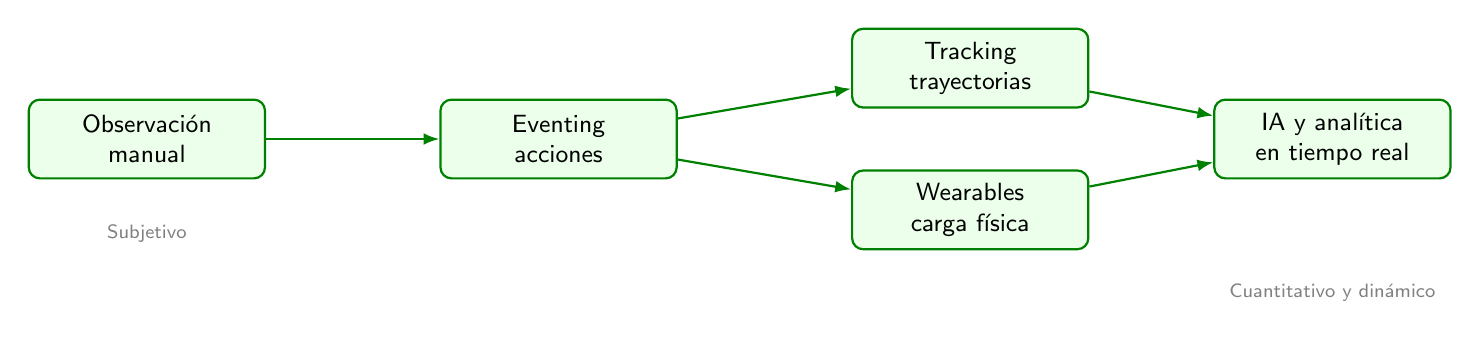
\begin{tikzpicture}[
		evol/.style={
			rectangle,
			rounded corners=4pt,
			draw=green!50!black,
			thick,
			fill=green!8,
			minimum width=3.0cm,
			minimum height=1.0cm,
			align=center,
			font=\sffamily\small
		},		
		flecha/.style={
			-{Latex[length=2mm]},
			thick,
			green!50!black
		}
		]
		% Nodes
		\node[evol] (obs)
		{Observación\\manual};
		\node[evol, right=2.2cm of obs]
		(event)
		{Eventing\\acciones};
		\node[evol, right=2.2cm of event, yshift=0.9cm]
		(track)
		{Tracking\\trayectorias};
		\node[evol, right=2.2cm of event, yshift=-0.9cm]
		(wear)
		{Wearables\\carga física};
		\node[evol, right=6.8cm of event]
		(ai)
		{IA y analítica\\en tiempo real};
		% Arrows
		\draw[flecha] (obs) -- (event);
		\draw[flecha] (event) -- (track);
		\draw[flecha] (event) -- (wear);
		\draw[flecha] (track) -- (ai);
		\draw[flecha] (wear) -- (ai);
		% Labels
		\node[
		font=\sffamily\scriptsize,
		text=gray,
		below=0.45cm of obs
		]
		{Subjetivo};
		\node[
		font=\sffamily\scriptsize,
		text=gray,
		below=1.2cm of ai
		]
		{Cuantitativo y dinámico};
	\end{tikzpicture}
\end{document}




\end{document}




